\section{Introduction}
\label{sec:intro}

\begin{figure*}[t]
  \centering
  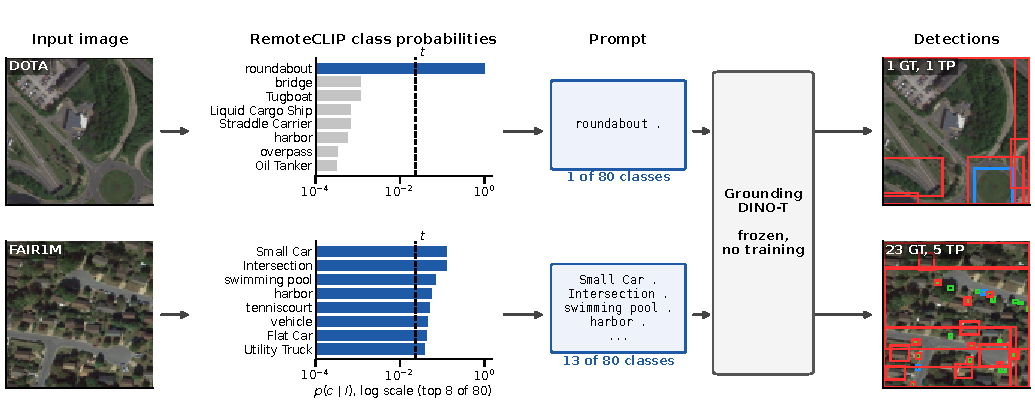
\includegraphics[width=\textwidth]{fig/pipeline.pdf}
  \caption{Overview of our training-free selector on two real dev images. RemoteCLIP turns the pixels into a probability for each of the 80 class names, and every class above the calibrated threshold $t$ (dashed line) goes into the prompt of the frozen detector. A confident image (top, DOTA roundabout) keeps a single class, an ambiguous residential scene (bottom, FAIR1M) keeps 13. Blue bars are kept classes; only the 8 most probable classes are drawn. In the output panels green boxes are ground truth, blue are true positives and red are false positives at score $\geq0.14$.}
  \label{fig:pipeline}
\end{figure*}

Open-vocabulary object detection (OVD) lets the user decide at test time which classes the detector should look for, simply by writing their names \cite{liu2024grounding}.
For natural images this works surprisingly well.
Remote sensing imagery is a different story.
Aerial images contain many small and densely packed objects seen from the top, and the class lists of remote sensing benchmarks are long and full of near duplicates.
\lae \cite{pan2025lae}, for instance, contains \emph{vehicle}, \emph{small car}, \emph{passenger car} and \emph{van} at the same time.
When all such names are put in one prompt, the detector has to divide its confidence among look-alike names and the result is very poor: LAE-DINO \cite{pan2025lae} reports only 0.1 mAP for a \gdino-T pretrained on natural images.

The text prompt is not a passive filter in these models.
In \gdino the class names enter the feature enhancer, the query selection and the decoder, so they change the visual features themselves \cite{liu2024grounding,fu2026wedetect}.
Work on natural images also shows that the class text steers box regression, so a wrong name can pull the box onto the wrong object \cite{wang2023condhead}, and that overlapping concepts split the probability mass of a classifier \cite{li2024lbp}.
A long vocabulary also costs time, because a fusion detector has to run its text--image fusion again for every chunk of the prompt (31 passes for the 1,203 LVIS classes in \cite{fu2026wedetect}).
Hence, for a frozen detector, choosing the vocabulary is the main control that the user still has over the output.

How much does it matter on aerial data?
A recent zero-shot study \cite{tsourveloudis2026ovd} found that prompting \gdino with only the ground-truth classes of each \lae image raises F1 by about 15$\times$, and it lists vocabulary filtering as an open direction.
That number comes from an oracle that reads the labels, so it shows the headroom but it is not something one can deploy.

The natural next step is to look at the image first, guess which classes are present, and prompt the detector with only those.
The idea by itself is not new.
VocAda \cite{liu2025vocada} adapts the vocabulary per image at test time with a captioner (LLaVA-Next-7B), a noun parser and a class selector, and reports consistent gains on COCO and Objects365.
However it was tested on natural images with Detic-style detectors, and it costs 5.6--10.7\,s and 17--31\,GB of GPU memory per image \cite{liu2025vocada}.
That is not practical for large aerial archives, and it does not even fit on the 8\,GB GPU we had.
SHiNe \cite{liu2024shine} and the fine-grained benchmark of Bianchi \etal \cite{bianchi2024devil} show from other angles that OVD detectors are sensitive to how the vocabulary is written and that they degrade when it contains irrelevant or hard-negative entries.
In our literature search (last repeated in October 2026) we could not find any study of a cheap, deployable per-image selector for a \emph{frozen} OVD detector on \emph{aerial} imagery.

In this work we build such a selector and we have tried to be careful with the evaluation, because early in the project we noticed that the benchmark itself has a trap.
\lae merges five source datasets that annotate \emph{disjoint} sets of classes, so a correct ``vehicle'' box on a FAIR1M image (where cars are labelled ``Small Car'') is counted as a false positive by standard COCO evaluation.
We therefore report a source-aware score next to the standard one, decided before any test run.
Our selector (\cref{fig:pipeline}) uses RemoteCLIP \cite{liu2024remoteclip} to score all 80 names from the pixels and keeps every name above one calibrated threshold, so a clear image gets a very short prompt and an ambiguous one gets a longer prompt.

Our contributions are as follows.
\begin{itemize}
    \item A training-free, pixels-only selector that picks a per-image vocabulary with RemoteCLIP and an \emph{adaptive} size controlled by a single calibrated threshold. It adds about 8\,ms per image and needs no change to the detector.
    \item An evaluation protocol for merged benchmarks: source-aware AP, a difference that is called robust only when a percentile bootstrap, a basic bootstrap and a per-class sign test all agree, and a test split that was used exactly once after every choice was frozen.
    \item On 2,862 held-out test images the selector improves AP50 by 5.3$\times$ (standard) and 2.7$\times$ (source-aware) over the full 80-class prompt, beats a fixed top-8 selector built on the same encoder, and makes the pipeline 1.21$\times$ faster.
    \item A clear map of where this works and where it does not. The gain holds on DIOR/DOTA-like data and transfers to NWPU VHR-10 \cite{cheng2014nwpu} untuned, but it is absent on FAIR1M and xView. Several extensions that we expected to help (crop evidence, uncertainty-aware retention, captions, synonym expansion) did not improve detection, and we report them as negative results.
\end{itemize}
